\subsubsection{UCS 6 - Monitoraggio di una organizzazione}

\begin{figure}[h]
	\centering
    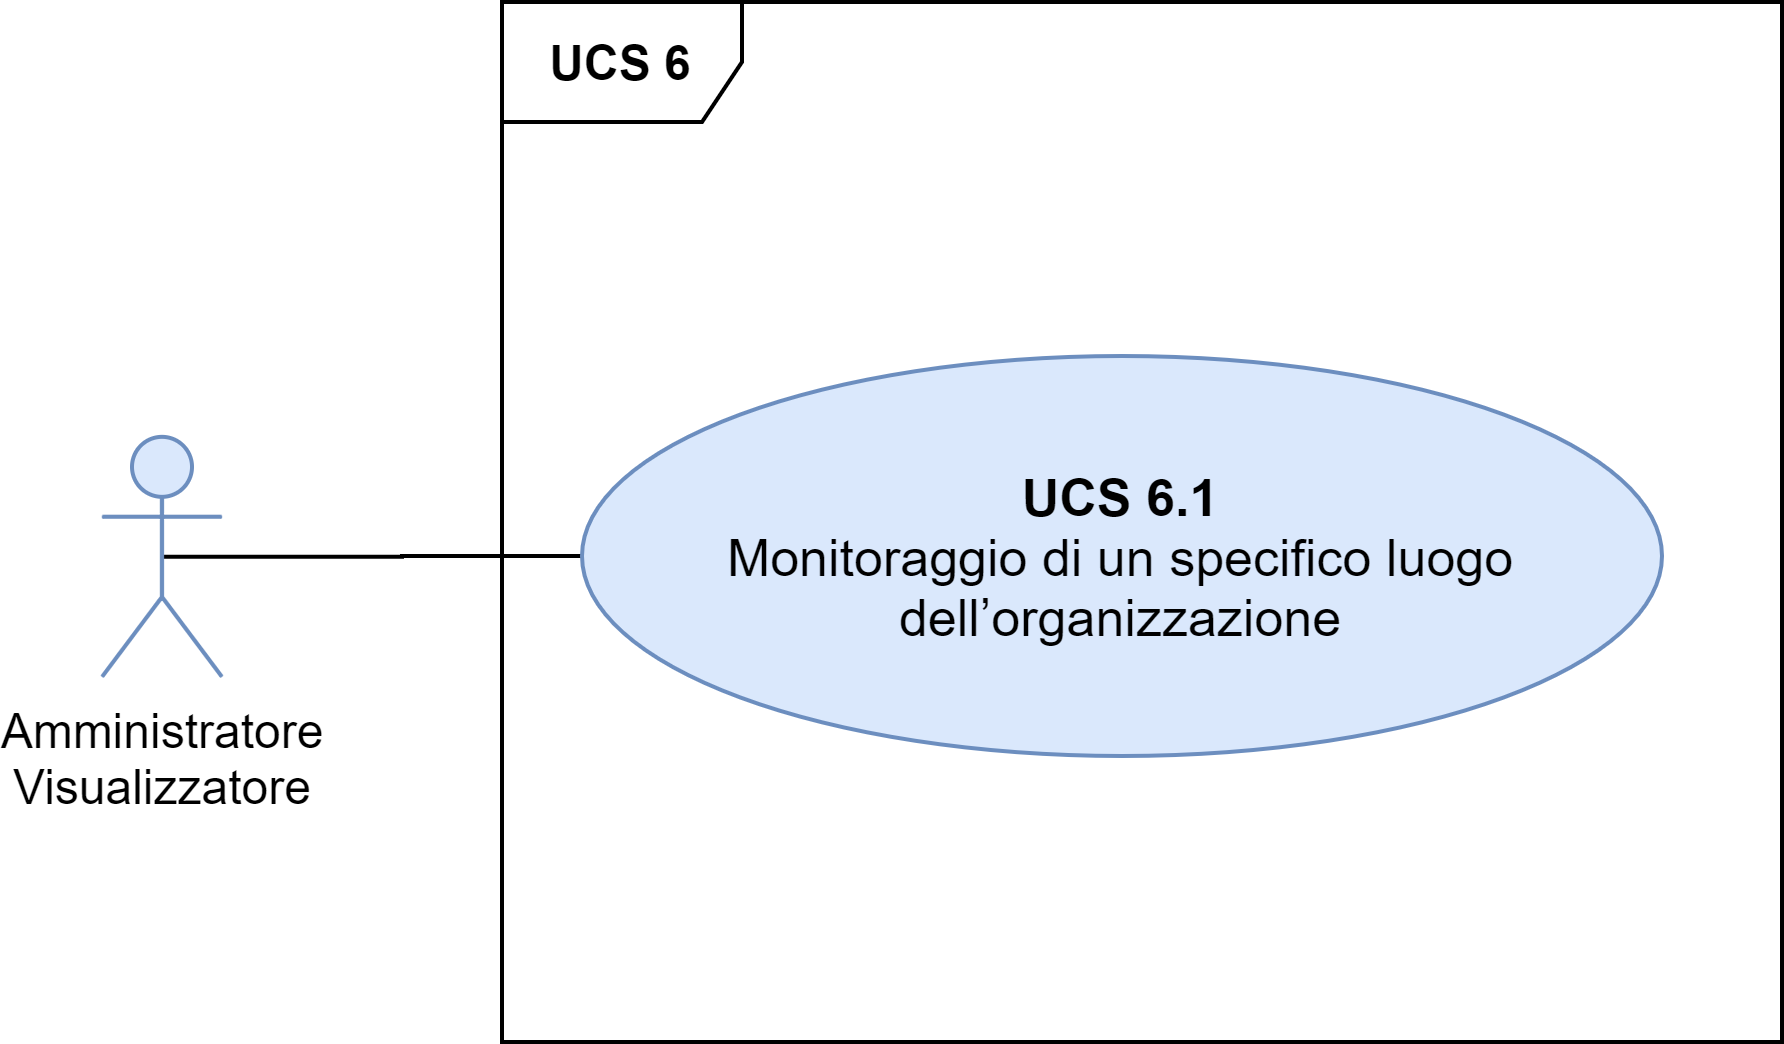
\includegraphics[scale=0.50]{Sezioni/UseCase/Immagini/UCS6.png}
    \caption{UCS 6 - Monitoraggio di una organizzazione}
\end{figure}

\begin{itemize}
	\item \textbf{Attori primari:} Amministratore visualizzatore
	\item \textbf{Precondizione:} L'amministratore dispone di almeno un'\glo{organizzazione}.
	\item \textbf{Postcondizione:} L'amministratore ha visualizzato il numero di utenti anonimi presenti in una \glo{organizzazione}.
	\item \textbf{Scenario principale:} L'amministratore deve scegliere l'\glo{organizzazione} che vuole monitorare selezionando la funzionalità di monitoraggio. Successivamente potrà accedere alla funzionalità di monitoraggio dei singoli luoghi all'interno dell'\glo{organizzazione} [UCS 6.1].
	\item \textbf{Flusso di eventi:}
\begin{enumerate}
	\item L'amministratore seleziona l'\glo{organizzazione} [UCS 3]; 
	\item L'amministrazione seleziona la funzionalità di monitoraggio dell'\glo{organizzazione};
	\item L'amministratore visualizza il numero di utenti anonimi presenti all'interno dell'\glo{organizzazione};
\end{enumerate}
\end{itemize}

\subsubsection{UCS 6.1 - Monitoraggio di un specifico luogo dell'organizzazione}

\begin{figure}[h]
	\centering
    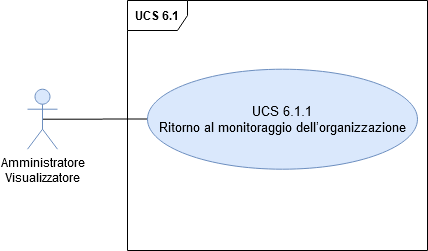
\includegraphics[scale=0.50]{Sezioni/UseCase/Immagini/UCS6.1.png}
    \caption{UCS 6.1 - Monitoraggio di un specifico luogo dell'organizzazione}
\end{figure}

\begin{itemize}
	\item \textbf{Attori primari:} Amministratore visualizzatore
	\item \textbf{Precondizione:} L'amministratore ha effettuato l'accesso alla funzionalità di monitoraggio dell'\glo{organizzazione}.
	\item \textbf{Postcondizione:} L'amministratore ha visualizzato il numero di utenti anonimi presenti in specifico \glo{luogo} dell'\glo{organizzazione}.
	\item \textbf{Scenario principale:} L'amministratore può monitorare un luogo all'interno dell'\glo{organizzazione} e ha la possibilità di tornare indietro al monitoraggio dell'intera \glo{organizzazione} [UCS 6.1.1].
	\item \textbf{Flusso di eventi:}
	\begin{enumerate}
	\item L'amministratore seleziona un luogo preciso da una lista contente tutti i \glo{luoghi} dell'\glo{organizzazione};
	\item L'amministratore visualizza il numero di utenti anonimi presenti all'interno di un specifico \glo{luogo} dell'\glo{organizzazione}.
	\end{enumerate}
\end{itemize}

\subsubsection{UCS 6.1.1 - Ritorno al monitoraggio dell'organizzazione}
\begin{itemize}
	\item \textbf{Attori primari:} Amministratore visualizzatore
	\item \textbf{Precondizione:} L'amministratore si trova all'interno della funzionalità di monitoraggio di un specifico luogo dell'\glo{organizzazione}.
	\item \textbf{Postcondizione:} L'amministratore ha effettuato l'accesso alla funzionalità di monitoraggio dell'intera \glo{organizzazione}.
	\item \textbf{Scenario principale:} L'amministratore ha scelto di tornare a monitorare l'intera \glo{organizzazione} e non solo parte di essa.
	\item \textbf{Flusso di eventi:}
    \begin{enumerate}
        \item  L'amministratore seleziona la funzionalità per tornare indietro a monitorare l'intera \glo{organizzazione}.
    \end{enumerate}
\end{itemize}
%\item L'amministratore seleziona da una lista contente tutti i \glo{luoghi} dell'\glo{organizzazione} uno preciso da monitorare;

%O creo un caso d'uso per visualizzare la lista dei vari settori 
%O metto nel 6.1 un flusso di eventi per dire che ho selezionato un elemento all'interno di quella lista
%O lascio così che sinceramente mi sembra andar bene, forse mi sfugge qualcosa